% !TEX root =  ../Report.tex

\chapter{Project Management}
\label{sec: Chapter 5}


\section{Project management methodology}

Due to the hybrid nature of our project, we wanted to ensure that we are able
to manage both the software and the theory aspect of the project effectively.
With respect to our software management, we primarily focused on a hybrid approach
with the help of a Kanban board, since we expected the core
set of requirements to change over time as we developed our theories and ideas.
An example of our Kanban board can be seen in figure \ref{fig:kanban},
where we split our requirements into categories.
Each category represents the state of a task, and is a common 
tool for tracking workload or the state of the project.


\begin{figure}[h!]
    \centering
    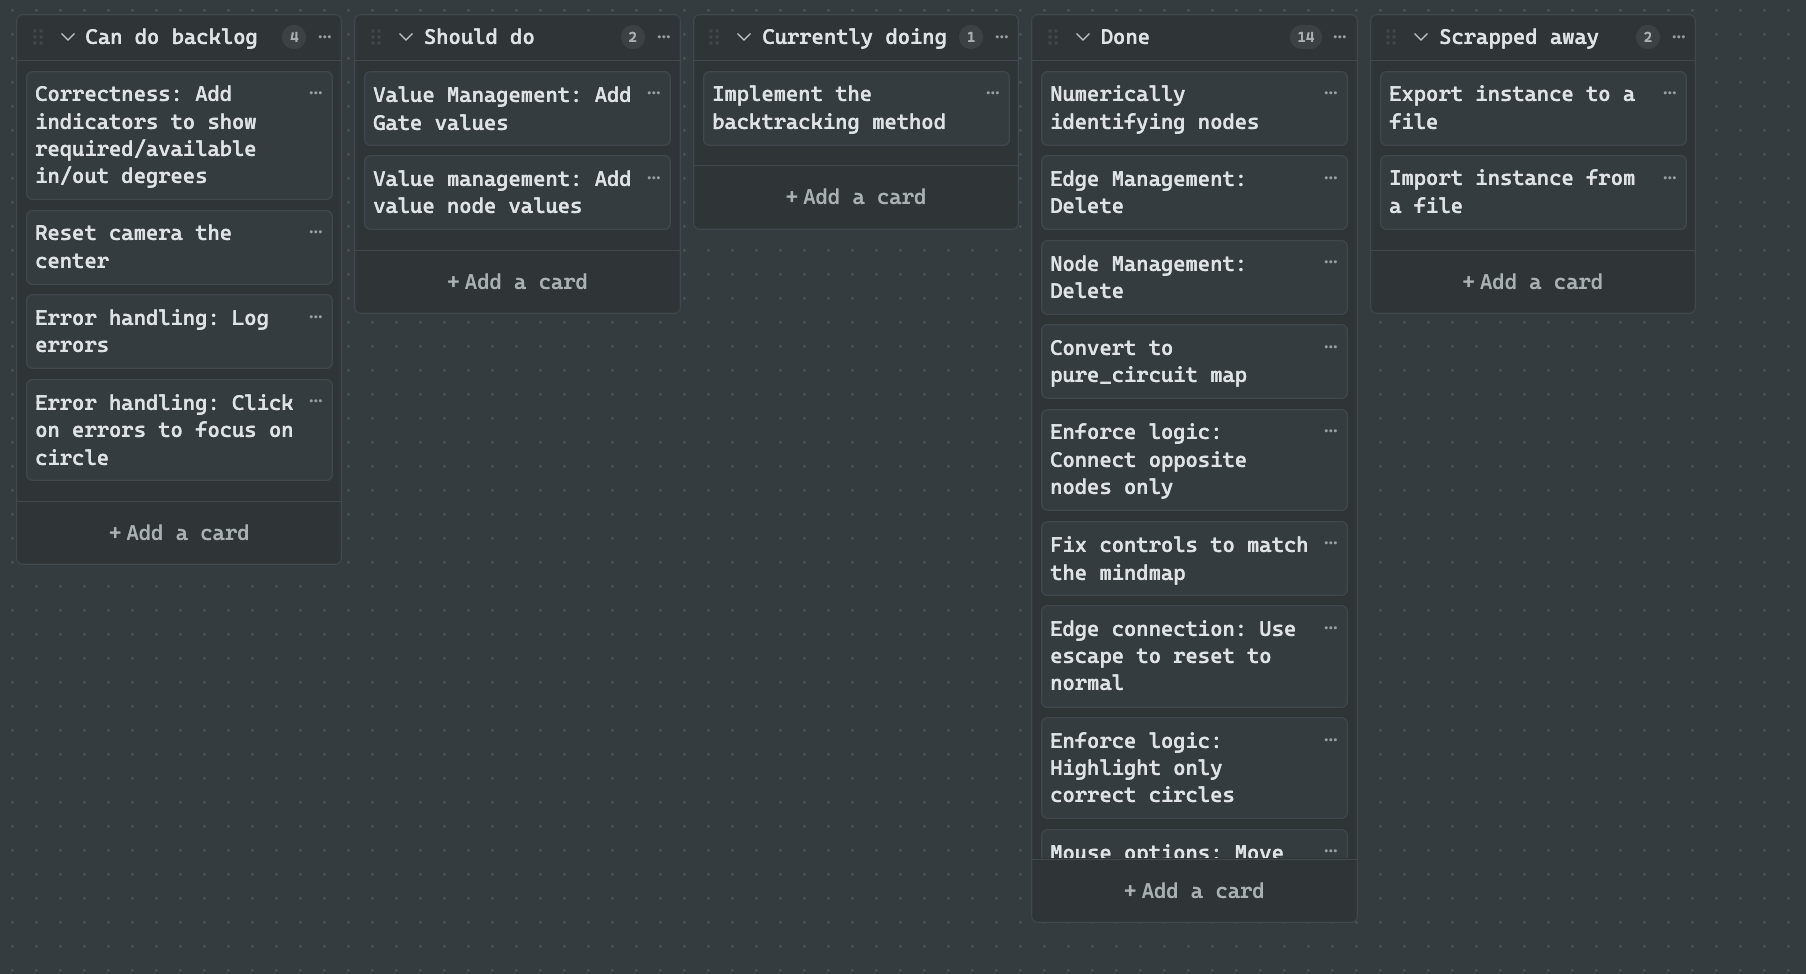
\includegraphics[width=0.7\textwidth]{Chapter5/kanban-board.png}
    \caption{Kanban board}
    \label{fig:kanban}
\end{figure}

With regard to the research management, we revolved our methodology around the \textit{Zettelkasten method}.
\textit{Niklas Luhmann} developed this method to keep track of notes and
information when dealing with a massive volume of publications  \cite{cevolini_ForgettingMachinesKnowledge_2018}.
The method embodies the following elements:
\begin{enumerate}
    \item \textbf{Literature Notes}: Atomic notes that have been extracted from literature which contain its ideas and techniques.
    \item \textbf{Fleeting notes}: Ideas that pop up randomly but are not linked with any particular source.
    \item \textbf{Permanent notes}: Reviewed literature notes and fleeting notes which have been promoted to
          \textbf{permanent} ones. These notes can be linked with other notes to create a web of knowledge.
\end{enumerate}
Each of these can be annotated with a tagging systems and relate to each other with the use of references.
Using the above method, we were able to extract ideas from different papers and create robust
theorems that are based off the current literature.

\section{Tooling}

To aid our research management, we made use of the \texttt{Obsidian} \footnote{https://obsidian.md/} tool.
\texttt{Obsidian}'s graphical representation of the semantical relations between nodes alongside its smart
tagging system, made it easier to keep track of our ideas and ongoing theories, as it is based
around the philosophy of the \textit{Zettelkasten method}.
Moreover, it incorporates additional features as seen in figure \ref{fig:theory:obsidian-usages},
such as a canvas or a mind-map. All these features allowed us to streamline and refine our theories
throughout the project.
In addition, to keep version control, we used \texttt{Github} \footnote{https://github.com/}
one of the most well known version control applications in industry.
This allowed us to keep constant backups of our code and notes and be able to
refer and revert to any changes made.


\begin{figure}[htbp]
    \centering
    \subfloat[Obsidian graph. Each dot represents a node and each link corresponds to a reference between two nodes]{
        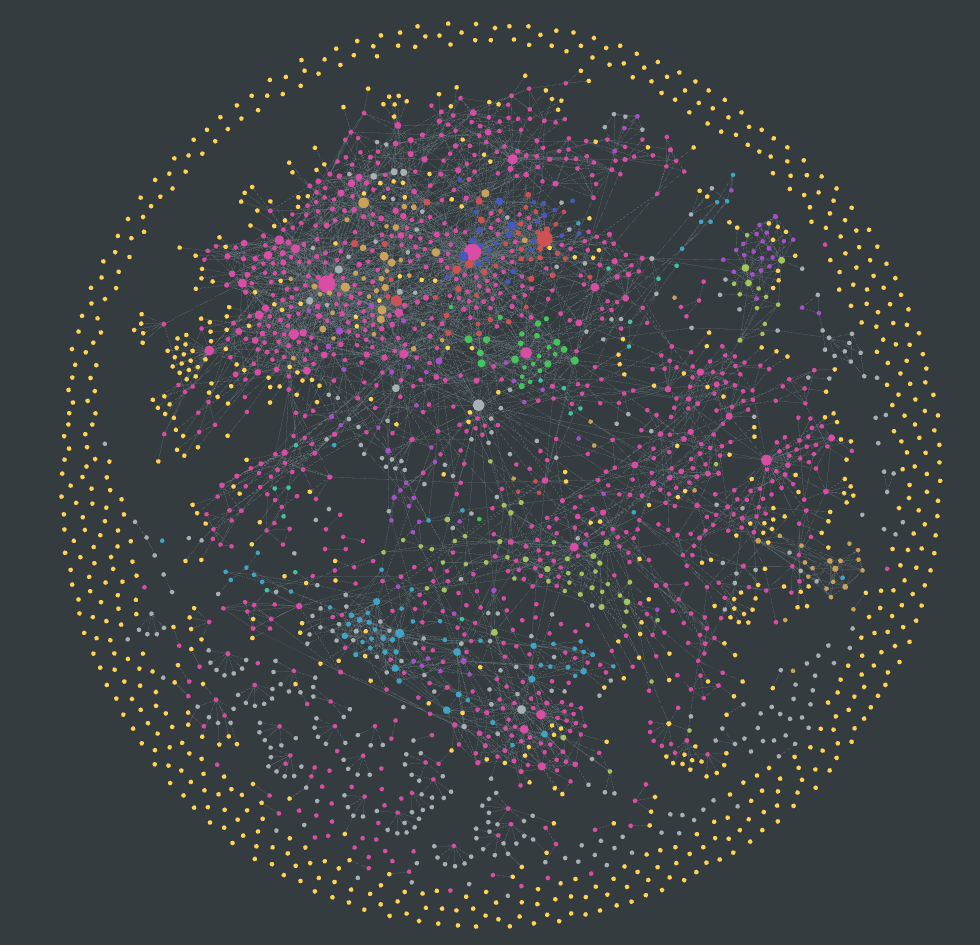
\includegraphics[width=0.3\linewidth]{assets/obsidian_graph.png}
        \label{fig:chap-5:obsidian-graph}
    }
    \subfloat[Obsidian Canvas]{
        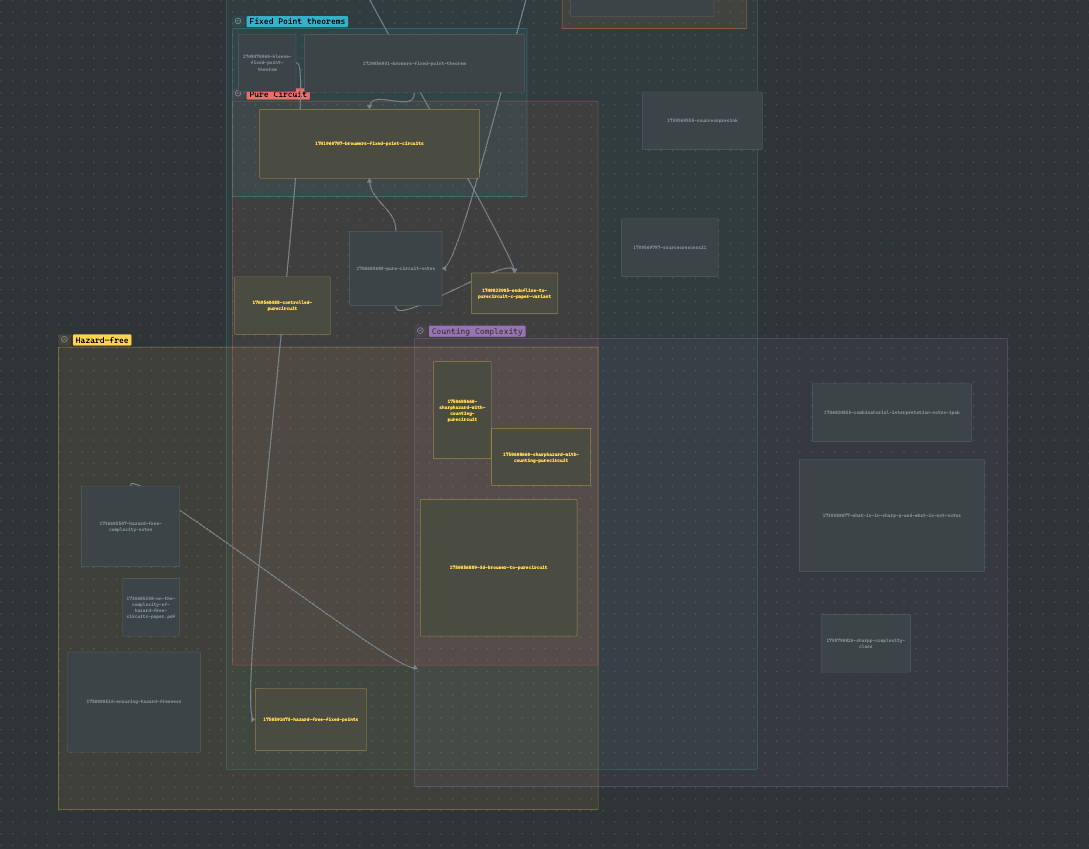
\includegraphics[width=0.3\linewidth]{assets/obsidian-canvas.png}
        \label{fig:chap-5:obsidian-canvas}
    }
    \subfloat[Obsidian mind-map]{
        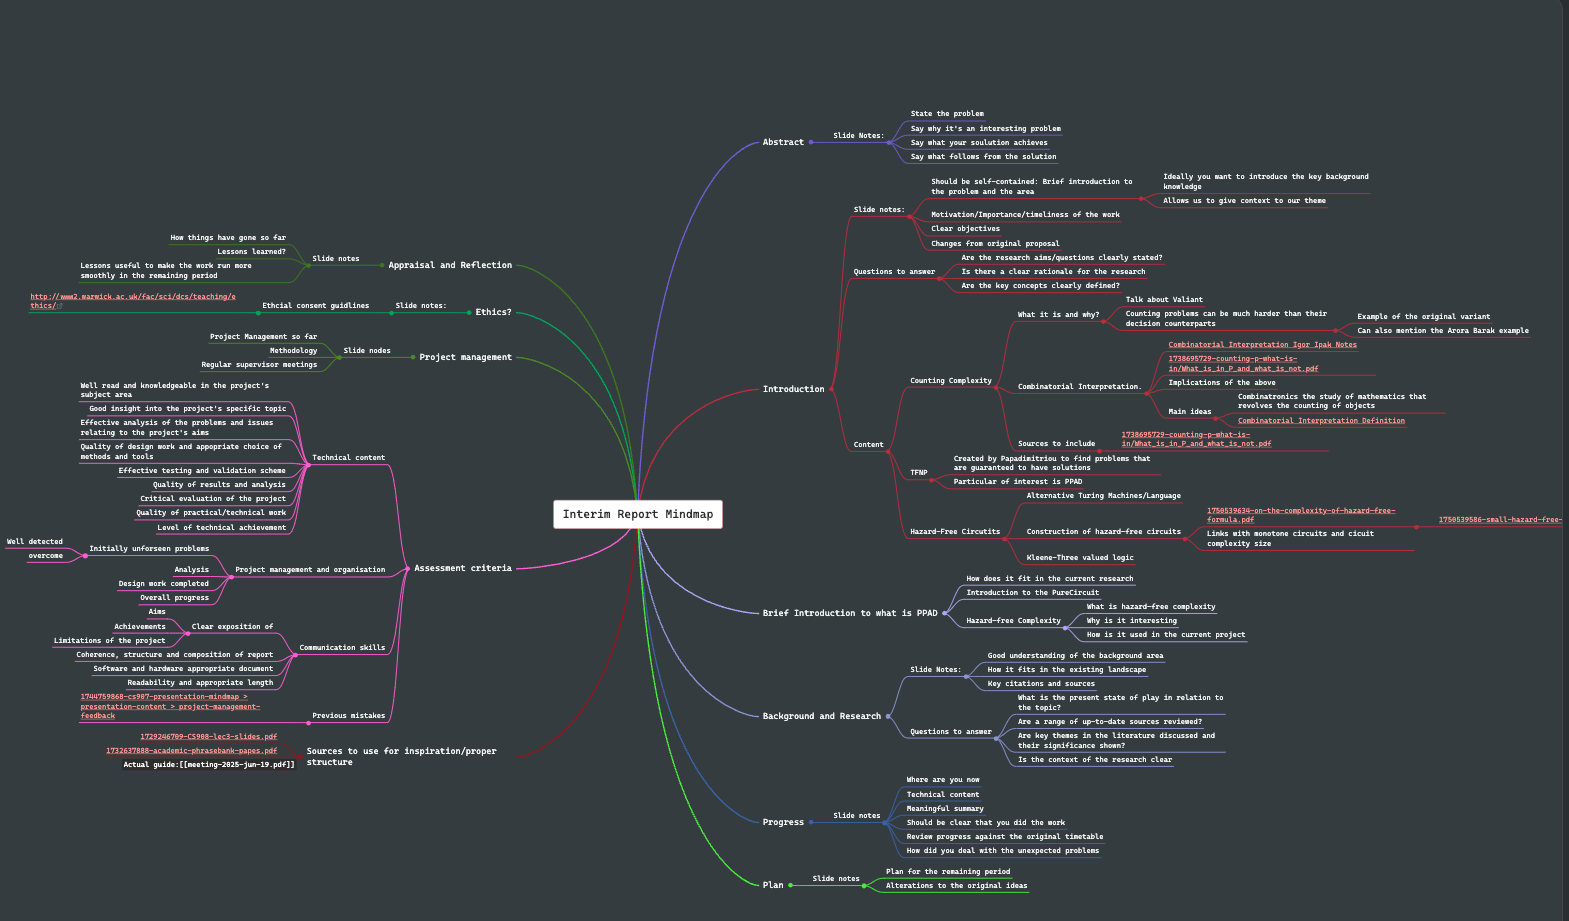
\includegraphics[width=0.3\linewidth]{assets/obsidian_mindmap.png}
        \label{fig:chap-5:obsidian-mindmap}
    }
    \caption[Usages of Obsidian]{Usages of Obsidian. Figure from interim report.}
    \label{fig:theory:obsidian-usages}
\end{figure}


\section{Ethical Considerations}

Due to the theoretical nature of the project, there were no ethical considerations
that were required. All data and diagrams that were referenced, were either made by the
author, redrawn by the author or referenced from another paper. The libraries
used to build the software were under the MIT licence and no third-party datasets were collected.

\section{Risk Assessment}
\label{sec:chap-5-risk-ass}

We provide a table of our current risk assessment in
the table \ref{tab:management:risk-management}. Overall through our extensive testing,
we were able to develop our algorithms fast enough without the worry of logic errors.
With respect to the theory crafting we faced several issues, as it was expected due
to the nature of the project. Moreover, the complexity of the milestones
and the difficulty of formulating sound proofs, required us to pivot to supplementary theorems
that will aid in the future resolution of the milestones. Due to our
robust note-taking system, we were able to implement the aforementioned strategy
without any significant hurdles.
We give our previous risk assessment table in the appendix \ref{sec:app:interim-risk},.


\begin{xltabular}{0.95\linewidth}{|Z{1.5cm}|Z{1.5cm}|Y|Y|Z{1.75cm}|}
    \hline
    \textbf{Severity} & \textbf{Prob} & \textbf{Description} & \textbf{Mitigation} & \textbf{Resolved} \\
    \hhline{|=|=|=|=|=|}
    High   & Medium & Software may not be feasible within the remaining time frame. & We focus on the validation and creation of instances.
    The current project is primarily research-based, and therefore we are mainly prioritising the theoretical development aspect. & \checkmark      \\ \hline
    Low    & Medium & Software not identifying a correct solution. & Usage of TDD techniques and property testing to ensure correctness.  Comparison with handmade instances. & \checkmark      \\ \hline
    Medium & High    & Difficulty of showing the parsimonious reduction from the  \textit{EndOfLine} to \textit{PureCircuit}. & Find parsimonious reductions from both directions.
    Reduce the overall reduction goal to a simpler one such as \textit{AntipodalSS} with \textit{HF-AntipodalSS}. &  \checkmark \\ \hline
    High   & High   & Inability to make significant progress on the \textit{SourceOrExcess} problems or the generalised statement. &
    Analyse the counting complexity of \textbf{PPAD}. Find parsimonious reductions from the \textit{SourceOrExcess} problem. & \checkmark \\ \hline
    High   & High   & Incorrect proofs or reductions. &
    Analyse the problem under different constraints.
    Apply the duck method, where we attempt to explain our ideas to an independent third-party. Validate proof with the supervisor or
    use the tool to investigate sample cases. & -  \\ \hline
    High   & Medium & Develop combinatorial-friendly variants of \textit{PureCircuit}. & Apply robustness on the gate set of \textsc{PureCircuit}.
    Develop new gates or variants are easier to work with or focus
    on a subset of solutions as explained in \ref{par:pure-circ-def}. & \checkmark  \\ \hline
    \caption{Risk management table.} \label{tab:management:risk-management}
\end{xltabular}




\section{Timetable}


We provide a figure of our final iteration of our Gantt chart in \ref{fig:gantt-new}
and the Gantt chart from our interim report in appendix \ref{sec:app:interim-report-gantt}.
Overall there were substantial changes as we shifted our
attention into the completion of the \textit{PureCircuit} tool
and the development of the necessary algorithms.

Due to complications that arose shortly after the interim report,
as mentioned in our risk assessment section \ref{sec:chap-5-risk-ass}, we shifted focus
to the topological interpretations of superpolynomial graphs
with polynomial degrees. This is also one of the reasons
why the software development was finished this late in the project.
We expand on this matter in greater detail in our section \ref{sec:app-and-ref}.
Overall, the project was completed within the expected timeframe
with the full software delivered as anticipated.



\begin{figure}[h!]
    \centering
    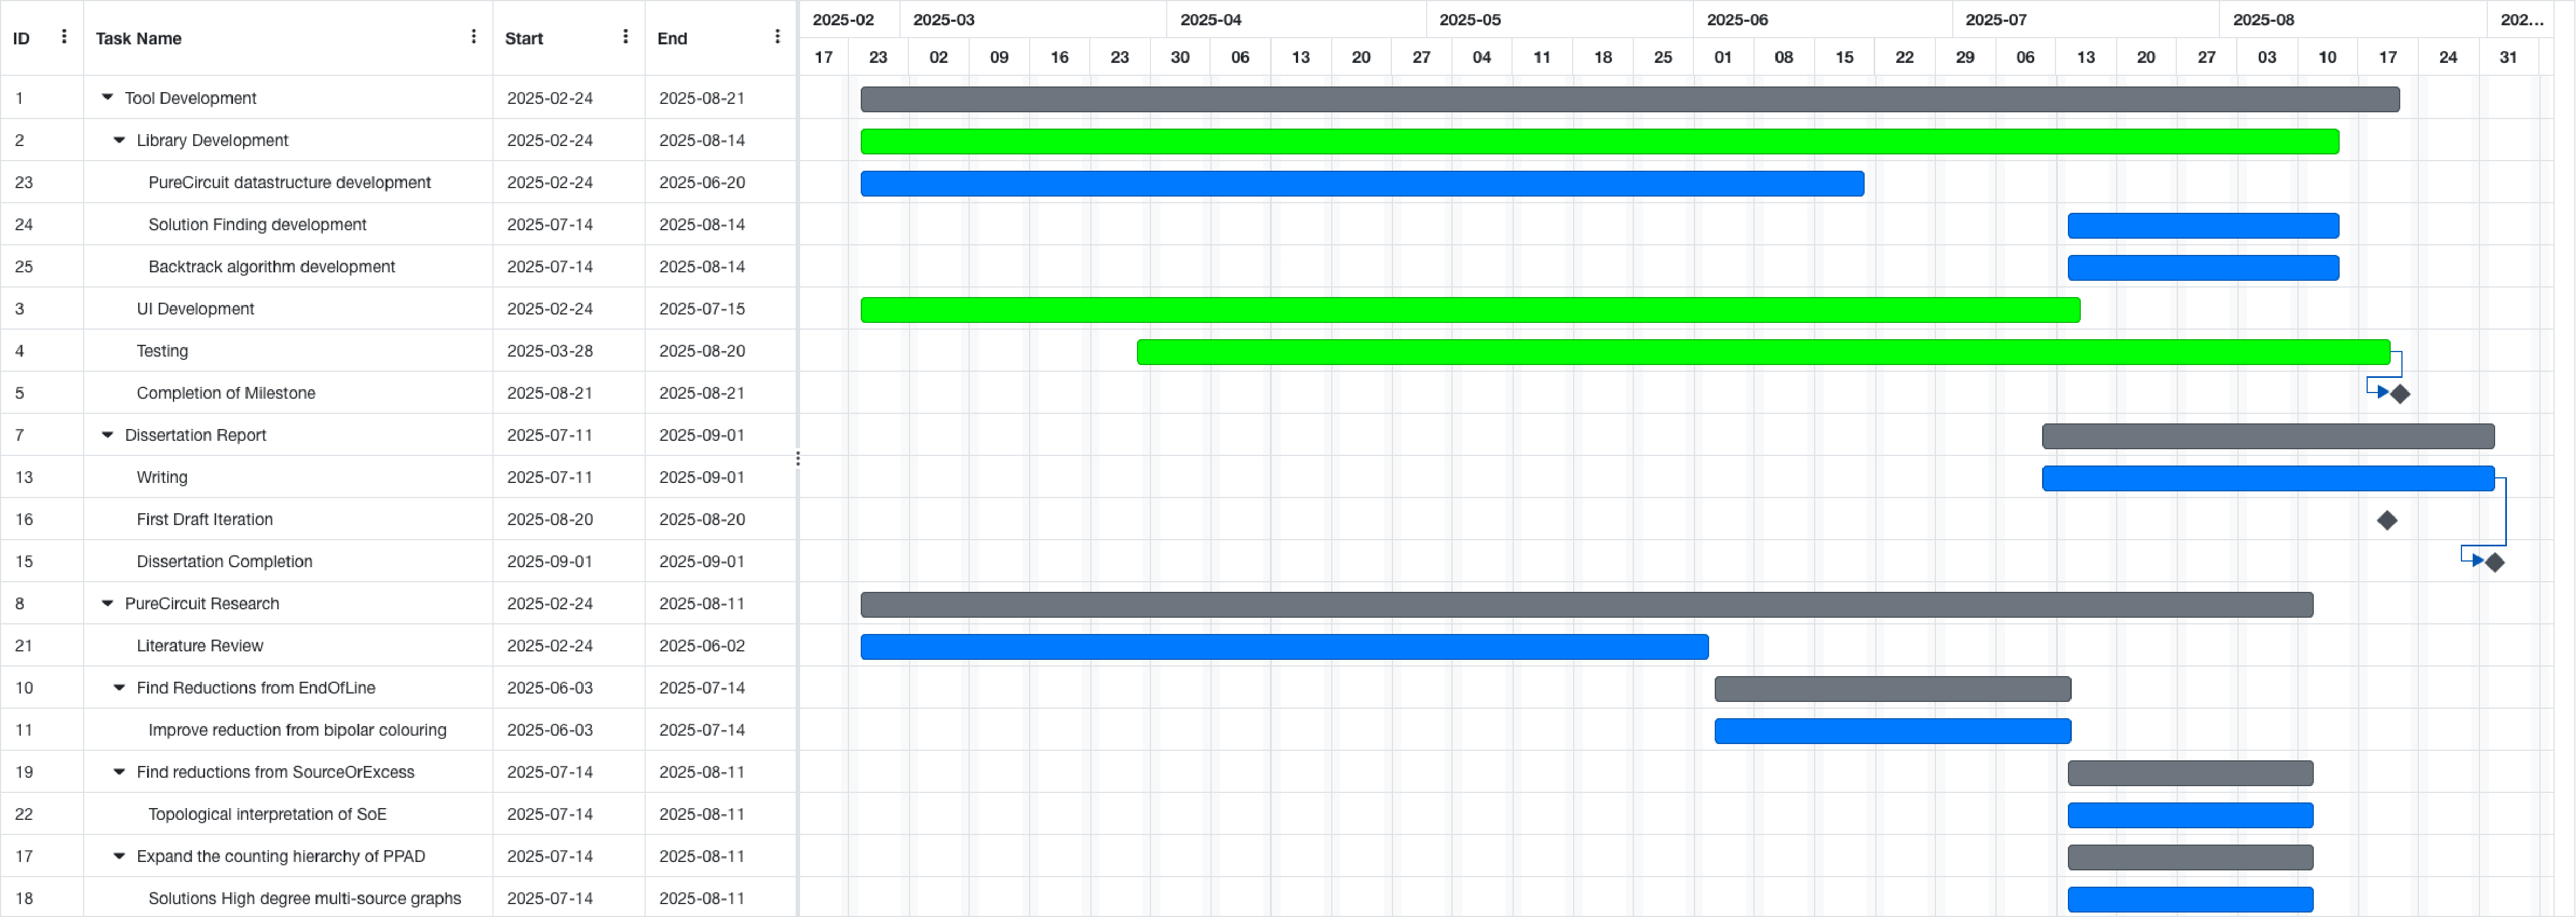
\includegraphics[width=0.95\linewidth]{gantt/gantt-pdf.pdf}
    \caption{Final Gantt chart}\label{fig:gantt-new}
\end{figure}

\section{Appraisals and Reflections}
\label{sec:app-and-ref}

As with any project, there were some aspects that proceeded as anticipated coupled with
several unexpected challenges.
First, a minimum viable version of the software was
completed much later than anticipated. Ideally, it would have been more beneficial for the project,
had we prioritised the development of the visualisation tool
as it would have allowed for faster verification
and prevention of incorrect theorems.
Moreover, one of our key results from the interim
report ended up having major issues that halted our progress,
which would have been prevented, had the tool been completed on time.

Fortunately, our rigorous testing methodology enabled us to complete the software development without encountering any major issues.
Additionally, our systematic note-taking process proved invaluable when handling unforeseen incidents,
allowing us to pivot from our research objectives effectively and explore alternative approaches such as topological interpretations
and multi-source graph problems.
This comprehensive documentation system also enabled us to learn from previous attempts
and refine our current results with greater certainty.
Many of our unsuccessful experiments ultimately contributed to our breakthrough results,
particularly in the main proofs presented in sections \ref{sec:pc-plus-eol} and \ref{sec:sc-excess}.


In summary, the project proved to be highly fulfilling. The opportunity to work in the intersection
of many well-studied fields allowed me to explore each one individually as well as
experiment with a variety of approaches. This offered me valuable
experience in research-based projects and improved important skills such us mathematical rigour.
Moreover, it taught me how to organise a project and
prioritise its components in order to ensure its success.
This project truly shaped my view of computer science and
my ambitions as a future researcher. Moving forward,
I intend to make use of the skills and knowledge I acquired
to make meaningful contributions to the field of computer science.


% Due to the limited prior research on the counting complexity of $\textsc{\#TFNP} -1$,
% this project involves significant risks.
% Our justification for the proposed milestones was largely informed by existing knowledge regarding the complexity of circuit constructions.
% However, it remained entirely possible that our proposed reductions could prove to be infeasible.
% Furthermore, working with Kleene logic introduced additional complexity, and it could be the reason why
% establishing fully parsimonious reductions between the target problems may not be achievable.
% This is also the reason why we diverted our attention to bounded parsimonious reductions instead.
% A detailed overview of the associated risks and our proposed mitigation strategies is provided in the table \ref{tab:management:risk-management}.

